%---------------------------------------------------------------------------------------------------
% Hauptteil
%---------------------------------------------------------------------------------------------------
%\newpage
%%\part{Hauptteil}

% Kapitel 1: Von der Integration zur Inklusion - eine Begriffserkl�rung 
\chapter{Von der Integration zur Inklusion - eine Begriffserkl�rung}
  \section{Der Weg von der integrativen P�dagogik zur inklusiven P�dagogik}
    \begin{flushleft}
      Der noch relative neue Begriff Inklusion, ist derzeit Bestandteil heftiger Debatten in der Fach�ffentlichkeit - es zieht so wohl Bef�rworter als auch Gegner nach sich. Mitverantwortlich f�r diese Unstimmigkeiten sind sowohl die unterschiedlichen �bersetzungen und Ableitungen dieses Begriffes, als auch die konzeptionelle Unterscheidung zum Begriff Integration. Doch um Inklusion und ihre Verbindung zur Integration zu verstehen, ist f�rderlich wenn wir historisch einige Schritte zur�ck gehen.\citep[vgl.][S.~18f]{Gemeinsam2012}
    \end{flushleft}
    
    \begin{flushleft}
      \enquote{\textit{Mit dem Begriff der Inklusion verbindet sich in der Fr�hp�dagogik der Gedanke, allen Kindern das Aufwachsen in einer Kindertageseinrichtung zu erm�glichen.} (Zitat: \citep[vgl.][S.~9]{Mittendrin2011}}
    \end{flushleft}

    \begin{flushleft}
      Inklusion ist aus p�dagogischer Sicht keine Erfindung des 21 Jahrhunderts, den Weg f�r Inklusion bzw. Inklusionsp�dagogik ebneten die Integrationsbestrebungen der 1970er Jahre des letzten Jahrhunderts. Hier war das Bestreben, die gemeinsame Erziehung und Bildung von Kindern mit und ohne besonderen F�rderbedarf in Kindertagesst�tten und Schulen. Diesen Fortschritt verdanken wir Eltern, die f�r ihre Kinder das Recht erstritten Regelkindertageseinrichtungen besuchen zu d�rfen und nicht wie es �blich war, Kinder mit Behinderungen in Sondereinrichtungen unterzubringen.\citep[vgl.][S.~9]{Mittendrin2011}
    \end{flushleft}
    \newpage
    \begin{flushleft}
      Das Bestreben alle Kinder gemeinsam zu erziehen und zu bilden ist bis heute nicht voll und ganz umgesetzt worden. Zwar ist der Inklusionsanteil in Kindertageseinrichtung mit 61,5\% im Vergleich zu nur 18,4\% in der Schule\footnote{2 Grundschulen : 33,6\%, weiterf�hrende Schulen 14,9\% Inklusionsanteil= Anteil der Kinder mit sonderp�dagogischen F�rderbedarf, die mit Kindern ohne F�rderbedarf zusammen in den Bildungseinrichtungen sind} recht hoch, doch es sollte nicht aus den Augen verloren werden, dass der Exklusionsanteil in Kindertageseinrichtungen immer noch 38,5\% betr�gt\citep[vgl.][S.~16]{InkiKte2011}. Im Gro�en und Ganzen kann man sagen, dass der Elementarbereich, der Bereich des deutschen Bildungssystems ist, in dem Inklusion am weitesten fortgeschritten ist, wohingegen sie dann in den folgenden Stufen immer mehr abnimmt. Gr�nde liegen unter anderem darin, dass in der Primarstufe teilweise noch Schuleingangsuntersuchungen existieren, die wiedergeben, ob ein Kind schulf�hig ist und wenn dies nicht der Fall ist, wird dieses Kind entweder zur�ckgestellt oder in eine Sonderschule �berwiesen.\citep[vgl.][S.~15]{InkidFr2010}
    \end{flushleft}

  \section{Abgrenzung zur Integrationsp�dagogik}
    \begin{flushleft}
      Betrachtet man Inklusion bzw. inklusive P�dagogik unabh�ngig von den Debatten, so kann sie als Notwendigkeit f�r eine Neubetrachtung, Weiterf�hrung und Modifizierung von Integration gesehen werden.\citep[vgl.][S.~19]{Gemeinsam2012} Das Ziel von Integration ist es Kinder in das System zu holen, da davon einer Zwei-Gruppen-Klassifizierung ausgegangen wird. Au�erdem stellt die Integrationsp�dagogik das Kind mit besonderen Bed�rfnissen isoliert in den Mittelpunkt. Wohingegen Inklusionsp�dagogik von einer heterogenen (vgl. Abschnitt \ref{sec:2_2}) Lerngruppe ausgeht, die gemeinsame Interaktion ist hier das Ziel. Somit l�sst Inklusion es gar nicht so weit kommen, dass Menschen aus dem System ausgeschlossen werden.\citep[vgl.][]{DownSyndrom2012} Damit verk�rpert Inklusion genau das Gegenteil von Exklusion (Ausgeschlossensein). Eine weitere Form ist die Separation, ihr Ziel ist die h�chst m�gliche Homogenit�t von Gruppen. Ein Produkt der Separation ist die Sonderp�dagogik. Diese stellt sich in folgender Abbildung dar:\citep[vgl.][S.~18]{Gemeinsam2012}
    \end{flushleft}
    
    \begin{center}
      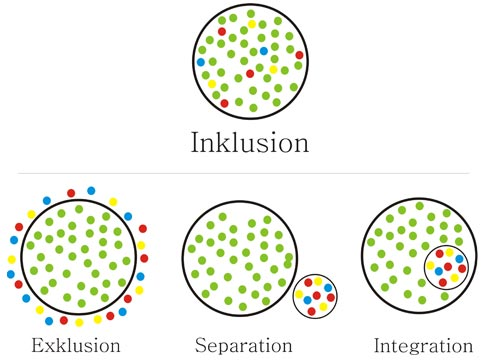
\includegraphics[width=.60\textwidth]{grafik/inklusion.jpg}
      \captionof{figure}[Die Abbildung stellt die verschiedenen Formen die Gesellschaft annehmen kann dar]{Die Abbildung stellt die verschiedenen Formen die Gesellschaft annehmen kann dar \citep[vgl.][]{Inkolpe2012}}
      \label{fig:inklusion}
    \end{center}
    
    \begin{flushleft}
      Des Weiteren geht Inklusion davon aus, dass alle Menschen ein Recht auf gemeinsame Erziehung und Bildung haben. Der Anspruch besteht darin Schulen und Kindertagesst�tten so zu gestalten und auszustatten, dass kein Kind bzw. Mensch (dies gilt auch f�r Mitarbeiter und Eltern) ausgeschlossen wird. Hierf�r ben�tigt es ein Zusammenspiel von vielen Parteien, denn jeder --- Kinder, P�dagogen, Eltern, Verwaltung und Politik tr�gt dazu bei, dass Inklusion  gelebt werden kann \citep[vgl.][S.~5]{IndexInk2007}. Obendrein verlangt Inklusion Ausgrenzung zu  vermeiden und Barrieren f�r Spiel, Lernen und Partizipation zu reduzieren. Bei der Vermeidung von Ausgrenzungen ist es wichtig niemanden in eine \enquote{Schublade zu stecken}, denn jedes Kind ist anderes und hat seine eigene Pers�nlichkeit und Begabungen. Jedes Kind bringt Erfahrungen und Eigenschaften mit, die es pr�gen und gepr�gt haben das macht jedes Kind einzigartigen. Doch die Einzigartigkeit kann sich nur in einer wertsch�tzenden Gemeinschaft bzw. Gesellschaft optimal entwickeln und entfalten. So ist das Ziel von inklusiver P�dagogik eine Gemeinschaft zu werden in der Heterogenit�t (vgl. Abschnitt \ref{sec:2_2}) als die Norm gesehen wird. Teilhabe und Chancengleichheit sind hier Schl�sselw�rter.\citep[vgl.][S.~9f]{Vielfalt2012}
      \newline
      Inklusion zu 100\% durchzusetzen und umzusetzen ist ein Ideal was nat�rlich erstrebenswert ist, aber bei l�ngerer Betrachtung nicht umsetzbar ist. Denn f�r eine v�llige Inklusion m�ssten alle Ausgrenzungsmechanismen und -prozesse verband werden. Dies scheint undenkbar, denn sowie auch inklusiven P�dagogik im st�ndigen Wandel ist, so sind auch Ausgrenzungsprozesse im st�ndigen Wandel und schwer zu �berwinden. Trotz allem sollte es aber nicht zur Resignation f�hren, sondern anspornen Inklusion zu leben.\citep[vgl.][S.~15]{IndexInk2007}
    \end{flushleft}


\newpage

% Kapitel 2: Fehldeutungen und Chancen von Inklusion				
\chapter{Fehldeutungen und Chancen von Inklusion}
  \section{Rechtliche Grundlage}
    \begin{flushleft}
      Erste Schritte und Rahmenbedingungen f�r Inklusion zu schaffen und diese auch auf gesellschaftlicher Ebene zu erreichen, gelang im Verlauf der 2006 stattfindenden UNESCO- Weltmeisterkonferenz. Dies wurde als Auftrag an alle Mitgliedstaaten formuliert. In Deutschland wurden 2009 die Leitlinien f�r inklusive Bildung ver�ffentlicht.\citep[vgl.][S.~11]{Vielfalt2012} Die Umsetzung von inklusiver Fr�hp�dagogik verlangt mehr als nur eine rechtliche Entscheidung, sowohl auf nationaler, wie auch auf internationaler Ebene. Es wird vielmehr ein weites Spektrum an rechtlichen Dokumenten ben�tigt um diesem facettenreichen und komplexen Thema gerecht zu werden. Wichtig f�r Inklusive P�dagogik in Deutschland wie auch international sind die UN-Menschenrechtskonvention, die den Grundstein f�r Inklusion und inklusives Denken bildet. Des Weiteren spielen noch die UN-Kinderrechtkonvention, die UN-Behindertenkonvention, die UNESCO-Weltmeisterkonferenz und speziell f�r Deutschland das Kinder - und Jugendhilfegesetz eine wichtige Rolle.\citep[vgl.][S.~16]{InkidFr2010} Im weiteren Verlauf werde ich auf einige Punkte weiter eingehen und sie erkl�ren.
    \end{flushleft}
    \subsection{UN-Menschenrechtskonvention}
      \begin{flushleft}
        Die UN - Menschenrechtskonvention vom 10.Dezember 1948 ist das Fundament der inklusiven Bildung und Erziehung und wurde in weiteren Konventionen konkretisiert. Schon in der vom 10.Dezember 1948 verabschiedeten Resolultion 217 A (III) der Generalversammlung, ist Bildung ein Menschenrecht.\citep[vgl.][]{unmenschen2012}
      \end{flushleft}

    \subsection{UN-Kinderrechtskonvention}
      \begin{flushleft}
        Im Rahmen der UN-Kinderrechtskonvention, die am  20. November.1989 stattfand, wurde das �bereinkommen �ber die Rechte der Kinder verabschiedet.
        Die �bereinstimmung der Kinderrechtskonvention wurde von Deutschland 1990 unterzeichnet und trat dann im Jahre 1992 in Kraft.\citep[vgl.][S.~25]{Mittendrin2011}
        Doch die Fragen sind- Was besagt die Konvention und wie genau sehen die Rechte der Kinder aus? Verbot von Diskriminierung auf Grund von Behinderung von Kindern oder deren Eltern, Chancengleichheit unabh�ngig von Herkunft und sozialen Status. Au�erdem wird allen Kindern (Kinder mit Behinderungen sind damit ebenfalls gemeint) das Recht auf Bildung zugesprochen\citep[vgl.][]{unkinder1992}.
      \end{flushleft}
      \begin{flushleft}
        Bis zum Jahre 2010 behielt sich Deutschland vor Unterschiede bei der Umsetzung der Rechte inl�ndischer und ausl�ndischer Kindern zu machen. Hierbei f�hrte es zu einer starken Benachteiligung von Fl�chtlingskindern in vielerlei Hinsicht. Vor allem aber in den Bereichen Bildung, Kinder- und Jugendhilfe und medizinischer Versorgung. Von Chancenungleichheiten in den Bereichen Bildung und Ausbildung sind im gro�en Ma�e Kinder die von Armut betroffen sind, Kinder die von Behinderung betroffen sind und Kinder mit einem Migrationshintergrund betroffen. Hierf�r sprechen auch die Zahlen das nur 84\% von Kindern mit Migrationshintergrund eine fr�hp�dagogische Einrichtung besuchen.\citep[vgl.][S.~26]{Mittendrin2011}
      \end{flushleft}
      \begin{flushleft}
        Deutschland konnte trotz des Aktionsplans die Einhaltung und vollst�ndige Umsetzung der Kinderrechte nicht voll und ganz gew�hrleisten. Mit Schuld an der Misere ist die Nicht-Verankerung der Kinderrechte in der deutschen Verfassung, denn es verliert dadurch an Aufmerksamkeit des Staates und der Gesellschaft.\citep[vgl.][S.~26]{Mittendrin2011}
        \newline
        Am 1.August 2012 wurde ein Zusatzprotokoll erstellt, welches die Rechte der Kinder verbessern soll. Kinder und Jugendliche k�nnen auf internationaler Eben gegen den Staat bei Widrigkeiten gegen das Kinderrecht Beschwerde einlegen. Doch daf�r m�ssen mindestens 10 Staaten das Protokoll unterschreiben, damit es �berhaupt in Kraft tritt.
      \end{flushleft}
    \subsection{UN-Behindertenrechtskonvention}
      \begin{flushleft}
        In Deutschland wurde inklusive P�dagogik stark von den �bereinkommen der UN-Behindertenrechtkonvention beeinflusst \citep[vgl.][S.~9]{InkiKte2011}. Hier haben sich 2006 die Vereinten Nationen auf ein Abkommen geeinigt. Seit 2010 ist es auch auf Bundeseben rechtskr�ftig. Im Mittelpunkt der Behindertenrechtskonvention stehen die Chancengleichheit und die Diskriminierung von Menschen mit Behinderung. Sie lehnt damit an die Kinderrechtskonvention an bzw. f�hrt einige Punkte weiter aus.\citep[vgl.][S.~26]{Mittendrin2011}
        \newline
        Im Artikel 24 erkennen die Vereinten Nationen an, das Menschen mit Behinderungen ein Recht auf Bildung haben. Damit ein lebenslanges Lernen auch gew�hrleistet werden kann, versichern die Vereinten Nationen ein integratives  (im Englischen inclusive) Bildungssystem. Es geht bei der Konvention nicht darum Menschen mit Behinderungen einen Platz in der Gesellschaft und ihren Institutionen zu schaffen, es geht viel mehr darum die Gesellschaft und ihre verschiedenen Institutionen so zu gestalten, dass sie auf die Bed�rfnisse der menschlichen Vielfalt reagieren, agieren und diese anerkennen.\citep[vgl.][S.~27]{Mittendrin2011}
      \end{flushleft}
      \begin{flushleft}
        Erw�hnt werden muss, dass alle Vertragsstaaten zwar die Verpflichtung haben die Rechte in einem gewissen Rahmen umzusetzen, es aber nicht die M�glichkeit besteht diese einzuklagen solange es nicht auf Bundesebene umgesetzt wurde. Doch haben auch hier die Bundesl�nder wiederum verschiedene Vorgehensweisen bzw. Gesetzes�nderungen und somit sieht auch die Umsetzung unterschiedlich aus.\citep[vgl.][S.~16]{InkidFr2010}

        In Deutschland gehen rund die H�lfte der Kinder �ber drei Jahren mit besonderen F�rderbedarf in einen Regelkindergarten bzw. besuchen eine integrative Kindertageseinrichtung. Doch sieht man genauer hin, kann man gro�e Unterschiede in den einzelnen Bundesl�ndern erkennen\ref{fig:verteilung}. So besuchen in Th�ringen alle Kinder �ber drei Jahre mit besonderen F�rderbedarf, die eine Institution besuchen, eine integrative Kindertageseinrichtung bzw. einen Regelkindergarten wobei in Niedersachsen nur 42,1\% eine integrative Ma�nahme besuchen. Obwohl dies in Deutschland gesetzliche geregelt ist.\citep[vgl.][]{13kuj2009}
        \newline
        \enquote{\textit{F�r Kindertagesst�tten besteht �ber den Grundsatz der uneingeschr�nkten Teilhabe (� 4 Absatz 3, � 19 Absatz 3 SGB IX) hinaus ein integrativer F�rderauftrag (� 22a Absatz 4 Sozialgesetzbuch VIII). Demnach sollen Kinder mit und ohne Behinderung grunds�tzlich in Gruppen gemeinsam gef�rdert werden.}}(Zitat: \citep[][]{Unesco2012})

      \end{flushleft}
      \begin{center}
        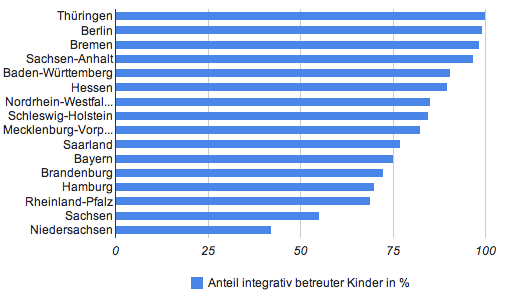
\includegraphics[width=.75\textwidth]{grafik/verteilung.png}
        \captionof{figure}[Verteilung integrativ betreuter Kinder �ber die deutschen Bundesl�nder]{Verteilung integrativ betreuter Kinder �ber die deutschen Bundesl�nder \citep[vgl.][]{13kuj2009}}
        \label{fig:verteilung}
      \end{center}
    \subsection{UNESCO Weltministerkonferenz}
      \begin{flushleft}
        Mit Teilnehmern aus mehr als 150 L�ndern fand 2008 die Abschlusssitzung der UNESCO Weltministerkonferenz zum Thema Bildung f�r alle in Genf statt. Es ist das gr��te und wichtigste Programm zum Thema Bildung. Das Ziel ist, dass alle Menschen zu einer qualitativ hochwertigen Bildung kommen, unabh�ngig  von Geschlecht, Hautfarbe, Religion, ihres sozio�konomischen Status\footnote{Der sozio�konomische Status bezeichnet Merkmalen menschlicher Lebensumst�nde. Dazu geh�ren beispielsweise: Bildung, Beruf, Besitz (auch kultureller Besitz) und Einkommen., url: \url{http://de.wikipedia.org/wiki/Sozio�konomischer_Status}} oder ihres besonderen F�rderbedarfs. Der Begriff Inklusion beschreibt und verk�rpert diesen Wunsch bzw. dieses Vorhaben am besten. Des Weiteren wird in der Abschlusserkl�rung der UNESCO Weltministerkonferenz, gefordert dass Bildungssysteme inklusiv sein sollen und das Bildungssysteme Vielfalt als Ressource sehen sollen.
        \newline 
         Die Leitlinien von dem Programm Bildung f�r alle unterst�tzen Staaten, Inklusion in ihrer Bildungspolitik und in ihren Bildungssystemen aufzunehmen . Die deutsche Fassung  \enquote{Inklusion: Leitlinien f�r die Bildungspolitik} macht die Erkenntnisse der internationalen Beratungen �ber inklusive Bildung in Deutschland zug�nglich. Obendrein bietet es einen �berblick �ber das Konzept der Inklusion sowie die rechtlichen Instrumente. Den Staaten werden  konkrete Leitfragen an die Hand gegeben. Diese geben Hilfestellung bei der Analyse des Bildungssystems. So kann z.B. Deutschland schauen wo es im Bildungssystem noch Verbesserungspotential gibt und wie der Wandel zur Inklusion vorrangetrieben werden kann. Des Weiteren wird aufgezeigt wie wichtig es ist, den Inklusionsgedanken in Deutschland zu st�rken.
         \newline
        Au�erdem besuchen ausnahmslos viele Kinder mit Migrationshintergrund F�rderschulen, die meist ohne ad�quaten Abschluss von der Schule abgehen. Folglich bleibt ihnen die Teilhabe und Chancengleichheit verweigert. Deutschland muss noch einiges Leisten um von einer Bildungsgerechigkeit in diesem Land sprechen zu k�nnen. Die UNESCO Leitlinien zeigen jedoch auf wie Deutschland dem Ziel von einer Inklusivenbildung n�her kommt.\citep[vgl.][]{UNESCO2010}
      \end{flushleft}
    \subsection{Gesetzliche Grundlagen in Deutschland}
      \begin{flushleft}
        In Deutschland bildet das am 1 Januar 1990 in Kraft getretene Kinder- und Jugendhilfegesetz (Achte Buch Sozialgesetzbuch (SGB VIII)) die Grundlage f�r einen deutschlandweiten gesetzlichen Rahmen der Kinderbetreuung. Das Kinder- und Jugendhilfegesetz regelt unter anderem die Bildung, Betreuung und Erziehung von Kindern in Kindertagesst�tten. Doch auch hier gibt es unterschiedliche Auslegungen in den sechzehn Bundesl�ndern. Zur Weiterentwicklung der Kinder und Jugendhilfe und zum Ausbau der Tagesbetreuung wurde das Tagesbetreuungsgesetz entwickelt.\citep[vgl.][]{Mittendrin2011} Das am 1.1.2005 in Kraft getretene Gesetz, dient unter anderem dem Ausbau der Betreuung von Kindern unter drei Jahren, h�heren Qualifikationsanforderungen und Qualit�tsentwicklung in der fr�hkindlichen Bildung.\citep[vgl.][]{TAG2004} Hervorgehoben werden die Verbesserungen und Bedeutung von Bildung, Erziehung und Entwicklung in der Fr�hp�dagogik. Dies soll Kindern gleichere Startbedingungen erm�glichen. Die Betreuungsquote der Kinder im Alter von unter drei Jahren ohne Migrationshintergrund liegt bei 30 Prozent. Bei Kindern mit Migrationshintergrund ist die Betreuungsquote mit 14 Prozent nicht einmal halb so hoch.\citep[vgl.][]{Dritter2012}
      \end{flushleft}
      \begin{flushleft}
        Eine weitere Gesetzs�nderung bildet in der Bundesrepublik einen zentralen Baustein beim Ausbau der Kindertagesbetreuung. Das am 16. Dezember 2008 in Kraft getretene Kinderf�rderungsgesetz (Kif�G) soll den Ausbau eines qualitativ hochwertigen Betreuungsangebotes beschleunigen, sowie ein bedarfsgerechtes und qualitativ hochwertiges Angebot f�r Kinder unter drei Jahren gew�hren.\citep[vgl.][]{BMFSFJ2010}
        Das Ziel ist es unter anderem, dass nach Abschluss der Ausbauphase (13. Juli 2013 ) ALLE Kinder unter drei einen Rechtsanspruch auf einen Betreuungsplatz haben. Von der Gesetzes�nderung sollen vor allem Kinder mit Entwicklungsgef�hrdung profitieren. Des Weiteren wird die Wichtigkeit der fr�hkindlichen Betreuung untermauert, sie verliert somit immer mehr ihren Stempel \enquote{nur eine Betreuungsst�tte} und erlangt den Status ein pr�ventive Funktion zu haben und als erste Bildungsst�tte. Kinder unter drei Jahren mit besonderen F�rderbedarf werden von dem Recht eine Regelkindertagesbetreuung besuchen zu d�rfen nicht ausgeschlossen.\citep[vgl.][S.~30f]{Mittendrin2011} Doch da stellt sich die Frage wie der Behinderungsbegriff in Deutschland definiert wird --- das Sozialgesetzbuch IX besagt: \enquote{Menschen sind behindert, wenn ihre k�rperliche Funktion, geistige F�higkeit oder seelische Gesundheit mit hoher Wahrscheinlichkeit l�nger als sechs Monate von dem f�r das Lebensalter typischen Zustand abweichen und daher ihre Teilhabe am Leben in der Gesellschaft beeintr�chtigt ist. Sie sind von Behinderung bedroht, wenn die Beeintr�chtigung zu erwarten ist.}( �2 Absatz 1 SGB IX,)\citep[vgl.][]{Beh2012}
      \end{flushleft}

      \begin{flushleft}
        Eine Behinderung wird bei Kindern unter drei eher selten diagnostiziert. Doch auch Kinder bei denen keine eindeutige Diagnose einer Behinderung vorliegt bzw. der Verdacht besteht von Behinderung bedroht zu sein, bekommen die gleichen Rechte wie Kinder die behindert sind.\citep[vgl.][S.~31]{Mittendrin2011} Hier wirkt der sonderp�dagogischer F�rderbedarf. F�r seine Feststellung muss ein Gutachten erstellt werden. Unter anderem wird festgelegt, ob und welche Ma�nahmen das Kind f�r eine uneingeschr�nkte Teilhabe in einer Kindertagesst�tte und f�r das sp�tere Leben ben�tigt.\citep[vgl.][]{Schul2012} In vielen Einrichtungen bietet der sonderp�dagogische F�rderbedarf ebenfalls kulturelle und politische Rahmenbedingungen und beeinflusst deren Handhabe. Auf diese Weise werden Gutachten �ber sonderp�dagogischen F�rderbedarf genutzt um individuelle F�rderpl�ne zu erstellen. Im Weiteren werden die Gutachten f�r Rechenschaftsberichte der Einrichtung �ber ihre Ausgaben f�r besonderen F�rderbedarf genutzt.\citep[vgl.][S.~17]{IndexInk2007}
      \end{flushleft}

  \section{Dimensionen -- ein Diskurs der P�dagogik der fr�hen Kindheit}\label{sec:2_2}
    \begin{flushleft}
      In Kindertagesst�tten ist eine Vielfalt an Pers�nlichkeiten vertreten, die alle zu ihrem Recht kommen wollen. Hierzu geh�ren nicht nur die Kinder die eine Einrichtung besuchen, sondern auch ihre Familien spielen eine zentrale Rolle im Heterogenit�tsverst�ndnis. Denn jede Familie bringt unterschiedliche Erwartungen, W�nsche, Vorstellungen und Erfahrungen und Lebensweisen mit, die sie von anderen unterscheidet und die sie gepr�gt haben. Dies bedeutet ein hohes Ma� an Qualit�t des Fachpersonals, um den Anforderungen gerecht zu werden. Dieser hohe Anspruch sollte nicht, als nicht zu erklimmender Berg gesehen werden, sondern als Chance wahrgenommen werden, der den p�dagogischen Alltag bereichert.\citep[vgl.][S.~37]{Mittendrin2011}
      Um Heterogenit�t zu verstehen, ben�tigt es eine Begriffserkl�rung. Heterogenit�t sollte nicht als Normabweichung sondern ganz einfach als Unterschiedlichkeit gesehen werden. Hier muss das vorherrschende Verst�ndnis von Norm und Normalit�t neu verstanden werden. Somit brauchen wir den veralteten Gedanken von Norm nicht als das was am h�ufigsten vor kommt zu verstehen, sondern das Normalit�t darstellt, dass jeder Mensch einzigartig ist und es somit nicht zwei gleiche Menschen gibt, sondern nur eine bunte Mischung aus vielen verschiedenen Pers�nlichkeiten.\citep[vgl.][S.~28]{Vielfalt2012}
    \end{flushleft}
    
    \begin{flushleft}
      Heterogenit�t zeigt sich in verschiedenen Dimensionen,
      \begin{itemize}
        \item Alter/Generationen,
        \item Schicht/Milieu,
        \item Gender,
        \item Kultur/Ethnie,
        \item Disability/Ability,
        \item Sexuelle Orientierung,
        \item Region,
        \item Religion und andere... (Zitat: \citep[][S.~21]{InkidFr2010})
      \end{itemize}

    auch wenn in der Fach�ffentlichkeit und im p�dagogischen Alltag haupts�chlich auf die vier Kategorien Migration, Behinderung, Geschlecht und sozialer Hintergrund eingegangen wird.\citep[vgl.][S.~37]{Mittendrin2011} Zwar sind solche Klassifizierungen unverzichtbar in Sozialeberichterstattung �ber Kinder, doch bergen sie auch Gefahren und Problem mit sich. Wie folgt kann es passieren, dass genau das Gegenteil von dem was inklusive Bildung verk�rpert passiert. Dem zu Folge kommt es dann zu  Stigmatisierung, Idealisierungen und Diskriminierungen, auch  wenn dies nicht beabsichtigt ist.\citep[vgl.][S.~21]{InkidFr2010}. Mit der Sensibilisierung f�r die Thematiken Diskriminierungskritik sowie Diversit�tsbewusstsein\footnote{Sich der menschlichen Vielfalt bewusstsein, url: \url{http://de.wikipedia.org/wiki/Diversity_Management}} wird noch einmal deutlich gemacht, wie wichtig es ist Kinder und ihre Familien nicht in eine Schublade zu stecken. Hier ist der Hinweis auf die Mehrfachzugeh�rigkeit eines jeden Kindes wichtig, damit P�dagoginnen nicht in die Falle von Differenz-Blindheit\footnote{Die Weigerung, Unterschiedlichkeiten zur Kenntnis zu nehmen.\citep[vgl.][S.~49]{Vielfalt2012}} oder Differenz-Fixierung\footnote{Einen Menschen auf Differenzen festlegen.\citep[vgl.][S.~49]{Vielfalt2012}} tappen.\citep[vgl.][S.~49]{Vielfalt2012} Deshalb ist es so bedeutend, dass das Fachpersonal sich bewusst ist, dass es nicht das Kind mit dem Migrationshintergrund gibt. Jedes Kind geh�rt noch weiteren Dimensionen an.\citep[vgl.][S.~38]{Mittendrin2011} Der kulturelle Hintergrund eines Kindes kann beispielsweise nicht ohne den Zusammenhang von Geschlecht, sozialen Status, Einkommen, Bildungshintergrund, Religion und Alter betrachtet werden.\citep[vgl.][S.~38]{Mittendrin2011} F�r die Umsetzung von inklusiver Bildung, ist es wichtig dass Fr�hp�dagogische Fachkr�fte sich bewusst werden, wie wichtige die eigene Sensibilisierung f�r die Verwobenheit der Unterschiedlichkeiten in einer Kita sind. Im weiteren Verlauf dieser Arbeit werde ich auch auf den p�dagogischen Umgang mit Vielfalt (Diversity Management) eingehen. In diesem Zusammenhang werde ich verschiedene Ans�tze betrachten.
  \end{flushleft}
  \newpage
  \section{P�dagogik der Vielfalt- Strategien zum Umgang mit Heterogenit�t im Praxisalltag}
    \begin{flushleft}
      Die Wertsch�tzung von individuellen Unterschieden wird im Deutschen mit dem Wort Vielfalt und im Englischen mit dem Wort Diversity ausgedr�ckt. Konzeptionell hat es sich in den Ans�tzen der P�dagogik der Vielfalt, Diversity Education oder auch des Diversity Management niedergeschlagen.\citep[vgl.][S.~21]{InkidFr2010}
    \end{flushleft}
    \begin{flushleft}
      Inwieweit Kinder Unterschiede anderer wahrnehmen, wurde noch nicht ausreichend wissenschaftlich untersucht. Daher stammt der Gro�teil der Erkenntnisse von Beobachtungen in Kindertageseinrichtungen. Trotz allem k�nnen diese Erkenntnisse Hinweise auf das Verhalten von Kindern geben. Das Wissen, welches Kinder �ber Unterschiede anderer haben, entwickelt sich sehr fr�h. Sie sind sich der Dominanzkultur\footnote{Dies bezeichnet den Teil einer Bev�lkerung, der aufgrund seiner quantitativen �berlegenheit die kulturelle Norm der Gesellschaft vorgibt, url: \url{http://de.wikipedia.org/wiki/Mehrheitsgesellschaft}} in der sie leben bewusst und k�nnen sich und andere in diese einbetten. Eigenschaften die Kinder wahrnehmen, sind unter anderem �u�ere Merkmale \enquote{Die sehen anders aus! Die sind nicht wie ich!} und Unterschiede in der Sprache.\citep[vgl.][S.~37ff]{Vielfalt2012} Um inklusiver Bildung und Erziehung gerecht zu werden, bedarf es einen sensiblen Umgang von fr�hp�dagogischen Fachkr�ften mit Vielfalt. Den Rahmen daf�r bietet unter anderen vorurteilsbewusste Bildung und Erziehung. Den Grundstein legte in den 1980ern das amerikanische Anti-Bias Approach. Der Anti-Bias Approach Ansatz geht davon aus, dass jeder Mensch vorurteilsbelastet ist und dass Vorurteile nicht als individuelle Fehlurteile gelten, sondern die Gesellschaft und ihre Institution dem Individuum diese vermitteln. Dementsprechend kann das Erlernte auch wieder verlernt werden und die Sicht auf menschliche Konstrukte ver�ndern. Das Projekt KINDERWELTEN hat diesen Ansatz f�r Deutschland adaptiert und hierzulande als Ansatz der Vorurteilsbewussten Bildung und Erziehung bekannt gemacht.\citep[vgl.][S.~43]{Vielfalt2012} Der Ansatz verfolgt, in Einbeziehung aller Dimensionen, vier Ziele die aufeinander aufbauen und essenziell f�r eine inklusive  Bildung und Erziehung sind.
    \end{flushleft}
    \newpage
    \begin{flushleft}
      \textit{\textbf{Ziel 1:} Jedes Kind muss Anerkennung und Wertsch�tzung finden, als Individuum und 
      als Mitglied einer bestimmten sozialen Gruppe dazu geh�ren Selbstvertrauen und 
      ein Wissen um seinen eigenen Hintergrund.}
      \newline\newline
      \textit{\textbf{Ziel 2:} Auf dieser Basis muss Kindern erm�glicht werden, Erfahrungen mit Menschen 
      zu machen, die anders aussehen und sich anders verhalten als sie selbst, so dass 
      sie sich mit ihnen wohl f�hlen und Empathie entwickeln k�nnen.}
      \newline\newline
      \textit{\textbf{Ziel 3:} Das kritische Denken von Kindern �ber Vorurteile, Einseitigkeiten und 
      Diskriminierung anzuregen hei�t auch, mit ihnen eine Sprache zu entwickeln, um 
      sich dar�ber verst�ndigen zu k�nnen, was fair und was unfair ist.}
      \newline\newline
      \textit{\textbf{Ziel 4:} Von da aus k�nnen Kinder ermutigt werden, sich aktiv und gemeinsam mit 
      anderen gegen einseitige oder diskriminierende Verhaltensweisen zur Wehr zu 
      setzen, die gegen sie selbst oder gegen andere gerichtet sind.
      (Zitat: \citep[][]{Kinderw2012})}
    \end{flushleft}
    \begin{flushleft}
      Doch wie l�sst sich dies umsetzten --- was muss eine Kita leisten um sich den Inklusionsprozess anzuschlie�en? Die Antwort darauf ist Vielfalt als Chance zu sehen. Die Kitas binden Vielfalt in ihren konzeptionellen Rahmen ein und unterst�tzend steht ihnen unter anderen der Index f�r Inklusion zur Seite\citep[vgl.][]{IndexInk2007}. Dazu geh�rt es das Team zu sensibilisieren. Die Mitarbeiter setzen sich mit Lebenswelten, Kulturen sowie Besonderheiten von Kindern und deren Familien auseinander. Mit der Bereitschaft anderen Lebenswelten und Familienkonstrukten aufgeschlossen zu begegnen. Hierbei sto�en sie auf schwierige und ungewohnte Aufgaben. Dieses gemeinsam zu reflektieren, kann hilfreich sein. Nicht alle Mitarbeiter haben immer die gleiche Meinung bei der Umsetzung und Auslegung von Inklusion. Doch die Teilhabe aller, barrierefreies Spielen, Lernen und Partizipieren, sowie interkulturelle Arbeit Grundpfeiler von inklusiver P�dagogik. Des Weiteren ist die Zusammenarbeit aller Beteiligten von gro�er Bedeutung f�r Inklusion. Die Basis ist eine verl�ssliche und offene Kommunikation aller Beteiligten. Denn Inklusion ist nicht nur neu f�r das Team, auch f�r die Familien ist es eine Herausforderung, die sie meistern und an der sie wachsen.\citep[vgl.][S.~200]{Vielfalt2012}\citep[vgl.][]{IndexInk2007}
    \end{flushleft}
    \begin{flushleft}
      Dass Inklusion mit den Eltern kommuniziert werden muss, wird in n�herer Zeit deutlicher werden. Die Umsetzung sollte dann nicht mehr schwer fallen --- doch es stellt sich die Frage wie sollen Kinder dies tun und was k�nnen sie dazu beitragen? In partizipativen Prozessen k�nnen Kinder, unabh�ngig von Alter und Entwicklungsstand, ihre Interessen und Bed�rfnisse einfordern, aber auch Ressourcen und Barrieren ihrer Einrichtung aufdecken, sowie gro�e und kleine Aufgaben im Kita Alltag �bernehmen. Die fr�hp�dagogische Fachkraft wird dann weniger zum Leiter und Vorreiter seiner Gruppe, sondern ist dann viel mehr Begleiter, Unterst�tzer, Herausforderer, Berater und Beobachter. Die individuellen Ressourcen werden dann als gro�e Bereicherung f�r die Einrichtung und f�r eine inklusive Bildung und Erziehung wahrgenommen.\citep[vgl.][S.~168]{Vielfalt2012}\citep[vgl.][]{IndexInk2007}
      Inwieweit sich das Streben nach einer inklusiven Fr�hp�dagogik verwirklichen l�sst, zeigt sich dann in den Spielsituationen der Kinder. Das besondere Augenmerk der fr�hp�dagogischen Fachkr�fte liegt hierbei darauf, ob alle Kinder die M�glichkeit zum gemeinsamen Spielen bekommen und inwieweit Kinder von Spielsituationen ausgeschlossen werden. Des Weiteren ist die Sensibilisierung f�r Ausgrenzungsprozesse und die Vermeidung von sozialer Exklusion in der Einrichtung ein Spagat, da Kinder in selbstbestimmten Interaktionen zu Exklusion neigen. Au�erdem beendet in der Regel das Eingreifen eines Erwachsenen die Spielsituation und das ausgeschlossene Kind bleibt in seiner Au�enseiterposition.
      Daher ist es die Aufgabe der fr�hp�dagogische Fachkraft sich als Br�cke zwischen den Kindern zu verstehen. Sie kann die Kinder bei sprachlichen �u�erungen unterst�tzen, ebenso k�nnen sie ihnen zeigen, wie sie Sprache als Kommunikationswerkzeug nutzen und in den gemeinsamen Spielprozess einsteigen k�nnen.\citep[vgl.][S.~76, 82]{Vielfalt2012}
    \end{flushleft}
    \begin{flushleft}
    \end{flushleft}           
\newpage

% Kapitel 3: Fazit				
%---------------------------------------------------------------------------------------------------
% Zusammenfassung
%---------------------------------------------------------------------------------------------------
% \newpage
%%\part{Schluss}
\chapter{Fazit}


\begin{flushleft}
In der Einleitung dieser Hausarbeit wurde darauf hingewiesen, dass die F�lle an Vielfalt sich nur entfalten kann, wenn allen die Chance an gesellschaftlicher Teilhabe und Teilnahme erm�glichen wird. Der Grundstein hierf�r sind gleiche Bildungschancen f�r alle. Doch wie ist es realisierbar?
\end{flushleft}


\begin{flushleft}
Die Hauptzielsetzung dieser Arbeit war es den Unterschied von Integration und Inklusion zu verdeutlichen. Dazu erfolgte zu erst die Beleuchtung des geschichtlichen Hintergrundes, sowie die Aufzeigung der Unterschiede zwischen Integration und Inklusion und welche Ver�nderungen es f�r das deutsche Bildungssystem bedeutet. Dem folgte die rechtliche und gesetzliche Auseinandersetzung mit dem Thema Inklusion, dies geschah sowohl auf der nationalen als auch auf internationalen Ebene. Zudem wurde der Begriff Heterogenit�t definiert und der Umgang mit Vielfalt wurde weiter er�rtert. Abschlie�end wurde auf die Frage eingegangen wie sich inklusive P�dagogik in der Praxis umzusetzen l�sst. 
\end{flushleft}

\begin{flushleft}
Durch die Hausarbeit k�nnte gezeigt werden, dass der Grundgedanke von Inklusion- die Einbeziehung und teilhabe aller- nicht neue ist. Den Grundstein legte in Deutschland, vor �ber vier Jahrzehnten, das Integrationsbestreben von Eltern. Sie k�mpften daf�r, dass ihre Kinder mit besonderen F�rderbedarf Regelkindertagesst�tten besuchen durften. Doch im Laufe der Jahre wurde immer deutlicher, dass das deutsche Bildungssystem nach mehr Ver�nderungen verlangt. Im Zuge dessen wurde der Integration Begriff durch den Begriff Inklusion abgel�st bzw. weitergef�hrt.
\end{flushleft}

\newpage
\begin{flushleft}
Erste Schritte im Entwicklungsprozess f�r eine inklusive P�dagogik wurden bereits vollzogen, doch sind wir lange noch nicht am Ziel angekommen. Zur Zeit wird zwar an vielen Kn�pfen gedreht um diesem Ziel einwenig n�her zu kommen, doch verlangt Inklusion mehr als neue politische Programme und Gesetze. Es gilt eine Haltung zu entwickeln und zu verinnerlichen, die Vielfalt als Chance und Ressource f�r Erziehung und Bildung von Kindern sieht. Hierf�r braucht es mehr Unterst�tzung von den Verantwortlichen, den Inklusion gibt es nicht zum Nulltarif. Au�erdem sollen Bedingungen geschaffen werden die es allen Beteiligten einfacher macht, dieses komplexe Thema anzugehen. Dem zu Folge sollte Inklusion, damit sie gelingt, nicht an der Kita T�r enden.
\newline\newline
\enquote{\emph{Wir m�ssen selbst die Ver�nderung sein, die wir in der Welt sehen wollen --- Mahatma Gandhi}}
% [Vielfalt2012, 73]
\end{flushleft}

\begin{flushleft}
Die Frage, die mich am Ende dieser Arbeit noch interessiert ist - Inwieweit muss sich die Ausbildung von fr�hp�dagogischen Fachkr�ften erweitern bzw. ver�ndern, damit sie allen Anforderungen, die inklusiver P�dagogik an das fr�hp�dagogische Fachpersonal richtet, gerecht werden kann? Die Auseinandersetzung mit dieser Frage, w�rde den Umfang dieser Arbeit �berschreiten. Es empfiehlt sich daher, dieses Thema in einer weiteren wissenschaftlichen Arbeit zu betrachten.
\end{flushleft}
           
\newpage

% Kapitel 4: Kinder der Regenbogengruppe				
% \chapter{Die Regenbogengruppe}
  \section{Anzahl, Geschlecht und Aufenthaltzeit}
    \begin{flushleft}
      In der Regenbogengruppe, die eine Integrationsgruppe ist werden zur Zeit 16 Kinder von einer Erzieherin, einer Heilp�dagogin und einer Kinderpflegerin betreut. Von den 16 Kindern drei Kinder �ber drei mit besonderen F�rderbedarf mit juristischer Anerkennung und ein Kind unter drei Jahren mit besonderem F�rderbedarf aber gegenw�rtig noch ohne juristische Anerkennung. Von den derzeitig 16 Kindern sind acht M�dchen und acht Jungen. Die Betreungszeiten der Kindern sind sehr unterschiedlich.  F�nf Kinder haben einen Platz von 8---12 Uhr, sieben Kinder haben einen Platz von 8---14 Uhr und vier Kinder werden nach Bedarf der Eltern an einigen Tagen von 8---12 betreut und an anderen von 8---14 Uhr. Allen Eltern steht frei, nach Bedarf Betreuungstunden f�r ihre Kinder dazu zu buchen. Der Gro�teil der Regenbogen-Kinder ist mit zwei oder drei Jahren in die Kindertagesst�tte Lotte Lemke gekommen. Sieben der Kinder der Regenbogengruppe waren zuvor bereits ein Jahr in der  Nachmitttagsgruppe (12---17 Uhr oder von 14---17 Uhr) und sind im August 2011 in die Regenbogengruppe gewechselt. Ein Kind ist seit seinem ersten Lebensjahr in der Gruppe. Au�erdem sind drei der Kinder erst mit vier Jahren in die Kindertagesst�tte Lotte Lemke gekommen.
    \end{flushleft}
    
    
  \section{Altersstruktur}
    \begin{flushleft}
      Das j�ngste Kind ist ein M�dchen, sie ist dieses Jahr zwei geworden. Da sie einen besonderen F�rderbedarf hat, ist sie nicht wie �blich bei Kindern unter drei in die Familiengruppe, sondern um dem besonderen Bedarf gerecht zu werden, in die Integrationsgruppe gekommen. Hier kann durch die Anzahl der Betreungskr�fte und der Heilp�dagogin ihr eher gerecht werden. Im Alter von drei Jahren sind zwei Jungen und ein M�dchen. Des weiteren gibt es drei vierj�hrige Jungen und drei vierj�hrige M�dchen. Vier Kinder der Regenbogengruppe sind f�nf Jahre alt, davon sind drei M�dchen und zwei Junge. Au�erdem gibt es noch zwei sechsj�hrige in der Gruppe, jeweils ein Jungen und ein M�dchen.
    \end{flushleft}           
% \newpage

% Kapitel 5: Familie				
% \chapter{Die Familien der Regenbogenkinder}
  \section{Die Familienkonstellation}
    \begin{flushleft}
      Fast alle Kinder der Regenbogengruppe leben in der traditionellen \enquote{Mutter- Vater-Kind-Familie}. Die Eltern eines M�dchens leben getrennt und sie lebt mit ihrer Mutter und Gro�mutter zusammen. Die Mehrheit der Kinder in dieser Gruppe,haben ein oder mehr Geschwister. Nur vier der Regenbogen-Kinder haben keine Geschwister. Von den Kindern mit �lteren Geschwistern besuchen zwei die Kita Lotte Lemke.  Einer geht ebenfalls in Regenbogengruppen und eine ist in einer der Familiengruppen. Alle anderen Kinder haben �ltere Geschwister die schon zur Schule gehen. Bei den Kindern mit j�ngeren Geschwistern ist es �hnlich. Hier besuchen ebenfalls zwei Geschwisterkinder die Kita. Eine davon ist in der Regenbogengruppe und der andere besucht eine der Elementargruppen. Alle anderen haben Geschwister, die noch nicht den Kindergarten besuchen. Familien mit mehr als zwei Kindern finden sich in drei F�llen. In zweien der F�lle sind die Geschwister �lter und in einem sind sie j�nger.
    \end{flushleft}

  \section{Berufst�tigkeit der Eltern}
    \begin{flushleft}
      Ein Gro�teil der Eltern ist berufst�tig bzw. ein Elternteil ist berufst�tig. In den meisten Familien kann man eine Tendenz zur klassischen Rollenverteilung erkennen. Acht M�tter haben sich aufgrund von kleineren Geschwistern bewusst entschieden noch nicht zu arbeiten, im Gegenzug dazu sind 14 V�ter berufst�tig und vollzeitbesch�ftigt. Von den berufst�tigen M�ttern, sind zwei vollzeitbesch�ftigt und drei teilzeitbesch�ftigt. Eine der berufst�tigen M�tter ist aufgrund ihrer Krebserkrankung bis auf Weiteres krankgeschrieben. Leider sind z.Z. bei zwei Kindern jeweils ein Elternteil ungewollt ohne Arbeit. 
    \end{flushleft}
    
    
  \section{Wohnsituation und Wohnort der Kinder}
    \begin{flushleft}
      Die meisten Kinder, der Regengruppe haben eine stabile Sozialelage. 
      Sie wohnen mit ihren Familien in Einfamilienh�usern mit Garten oder in Mehrfamilienh�usern und haben ihr eigenes Zimmer, ausgestattet mit den verschiedensten Spielsachen z.B. eine elektrische Eisenbahn, einen Kaufmannsladen, Murmelbahn oder auch ein Mischpult. Fast alle Kinder der Regenbogengruppe wohnen in der Gemeinde Halstenbek, zum Teil werden die Kinder zu Fu� oder mit dem Fahrrad in die Kita gebracht, aber der Gro�teil wird mit dem Auto gebracht.
    \end{flushleft}


  \section{Migration und besondere Bed�rfnisse}
    \subsection{Die F�rderung besonderer Bed�rfnisse}
      \begin{flushleft}
        Aufgrund des Integrationsstatus der Regenbogengruppe - wie bereits in 4.1 erw�hnt - sind hier drei mit Kinder �ber drei mit besonderen F�rderbedarf mit juristischer Anerkennung und ein Kind unter drei Jahren mit besonderen F�rderbedarf aber gegenw�rtig noch ohne juristischer Anerkennung. Au�erdem bekommen noch weitere Kinder eine besondere F�rderung. Derzeitig wird getestet, ob zwei Jungen eine Hochbegabung haben, diese Kinder haben besondere Bed�rfnisse, auf die eingegangen werden muss. Insbesondere erfolgt die Begleitung der Kinder mit besonderen Bed�rfnissen durch die Heilp�dagogin, die ein gro�es Augenmerk auf die Selbstverst�ndlichkeit im  Umgang mit Behinderungen jeglicher Art legt. \enquote{Jedes Kind ist besonders in seiner Art.} (Zitat: Britta Henningsen)
      \end{flushleft}

      \begin{flushleft}
         Da es eine Vielfalt von besonderen Bed�rfnissen gibt, arbeiten die P�dagogen mit einer Vielzahl an Therapeuten zusammen. Darunter fallen Ergotherapeuten, L�gop�den, Kinderpsychologen und Physiotherapeuten. Au�erdem wird mit verschiedenen Instituten, wie dem Werner Otto Institut und dem Fleming Institut, zusammengearbeitet \citep[vgl.][]{Integration2007}. Es besteht die M�glichkeit, dass externe Spezialisten in die Kindertagesst�tte kommen.
      \end{flushleft}

     
    \subsection{Migration und Sprachf�rderung}
      \begin{flushleft}
        Drei Kinder der Regenbogenkinder haben einen Migrationshintergrund (indisch, irisch und japanisch). Sie erhalten einmal pro Woche besondere Sprachf�rderung durch \gls{Sismik} (Sprachverhalten und Interesse an Sprache bei Migrantenkindern in Kindertageseinrichtungen). Diese F�rderung findet durch zwei p�dagogische Mitarbeiter, die beide eine Weiterbildung im Bereich Sprachf�rderung haben, statt. Dies findet zweimal die Woche w�hrend der AG-Zeit statt. Eine P�dagogin begleitet die 3 � j�hrigen bis 5 j�hrigen und eine andere die Kinder die dieses Jahr zur Schule kommen.
      \end{flushleft}           
% \newpage

% Kapitel 6: P�dagogische Arbeit				
% \chapter{P�dagogische Arbeit}
  \section{Der p�dagogische Auftrag der KiTa Lotte Lemke}\label{sec:7_1}
    \begin{flushleft}
        Der p�dagogische Auftrag der KiTa Lotte Lemke bezieht sich unteranderem auf den Bildungsauftrag vn INFANS-Konzept f�r Fr�hp�dagogik vom Institut f�r angewandte Sozialforschung / Fr�he Kindheit e.V.. Hier geht es vorallem darum, dass lernen ein  Lebenslanger Prozess ist, der von jedem Menschen mitbestimmt wird. Doch f�r eine gelungene Entwicklung sind Menschen abh�ngig,  von der Interaktion mit anderen. F�r das Kind hei�t das, es braucht eine Bindungsperson, um die Welt erkunden zu k�nnen \citep[vgl.][]{paBild2009}. Darauf aufbauend ist dem Personal der KiTa Lotte Lemke sehr wichtig, dass sich jedes Kind wohl und geborgen in der KiTa f�hlt und Vertrauen zu den P�dagogen aufbaut \citep[vgl.][]{paBild2009}. Jedem Kind wird Wertsch�tzung und Anerkennung entgegengebracht.
        \\
        Au�erdem ist dem KiTa-Team wichtig die Kinder mit wichtigen Attributen wie Selbstvertrauen, Selbstbewusstsein, Selbstst�ndigkeit, Konfliktf�higkeit, Entscheidungsf�higkeit, Toleranz und Akzeptanz, auszustatten \citep[vgl.][S.~12ff]{padZiel2000}. Des Weiteren sind die F�rderung der Kreativit�t und Phantasie f�r die individuelle Entwicklung und die F�rderung zur Entwicklung des Sozialverhaltens  wichtige Bestandteile des p�dagogischen Auftrags \citep[vgl.][S.~12ff]{padZiel2000}. \enquote{Hilf mir es selbst zu tun.} (Zitat: Maria Montessori zitiert nach \citep[vgl.][]{paBild2009}) 
    \end{flushleft}
  
  
  \section{Das Konzept und die Besonderheiten der KiTa}
    \begin{flushleft}
      Die KiTa Lotte Lemke die Schwerpunkten in ihrer Arbeit sind sehr verschieden unteranderem arbeitet die Kindertagesst�tte nach dem Situationsansatz. Die P�dagogen sind zu dem Entschluss gekommen, dass das gruppen�bergreifende Arbeiten die Merkmale des Situationsansatzes am Besten aufgreift. Durch Angebote, Projekte und AG's eignen sich die Kinder wichtige Attribute (vgl. Abschnitt \ref{sec:7_1}) an \citep[vgl.][S.~15f]{Sitans2000}.
    \end{flushleft}


    \begin{flushleft}
      Zudem ist das Thema Partizipation ein wichtiger Baustein im KiTa-Alltag. \enquote{Unter Partizipation verstehen wir die Mitbestimmung und Beteiligung der Kinder im Alltag.} (Zitat nach \citep[vgl.][]{Patiz2011}) Die Mitbestimmung ihres KiTa-Alltags erleben die Kinder t�glich. Ich m�chte dies an der t�glichen Bildertafel-Situation erl�utern. Die Kinder k�nnen  t�glich zwischen verschiedenen Angeboten, Projekten und AG's w�hlen. Dabei treffen sie nicht nur eigene Entscheidungen, sondern sie m�ssen sie sich auch untereinander abstimmen, da alle Angebote, Projekte und AG's nur eine bestimmte Kapazit�t haben. Hilfestellung von den P�dagogen sind hier dann auch angebracht \citep[vgl.][]{Patiz2011}. \enquote{Wir (P�dagogen) bestimmen, was Ihr (Kinder) bestimmen d�rft!} (Zitat nach \citep[vgl.][]{Patiz2011}) Wichtig ist zu erw�hnen das Partizipation nur im Zusammenspiel mit der Verfassung funktioniert (vgl. Anhang \ref{chap:anhang_5}). Die Verfassung, die 2007 in Kraft trat, beinhaltet die Partizipationsrechte der Kinder \citep[vgl.][]{Verfas2008}. 
    \end{flushleft}
    
    
  \section{Tagesablauf}
    \begin{flushleft}
      So k�nnte ein Tag in der Kindertagesst�tte Lotte Lemke aussehen.
    \end{flushleft}
    \begin{center}
      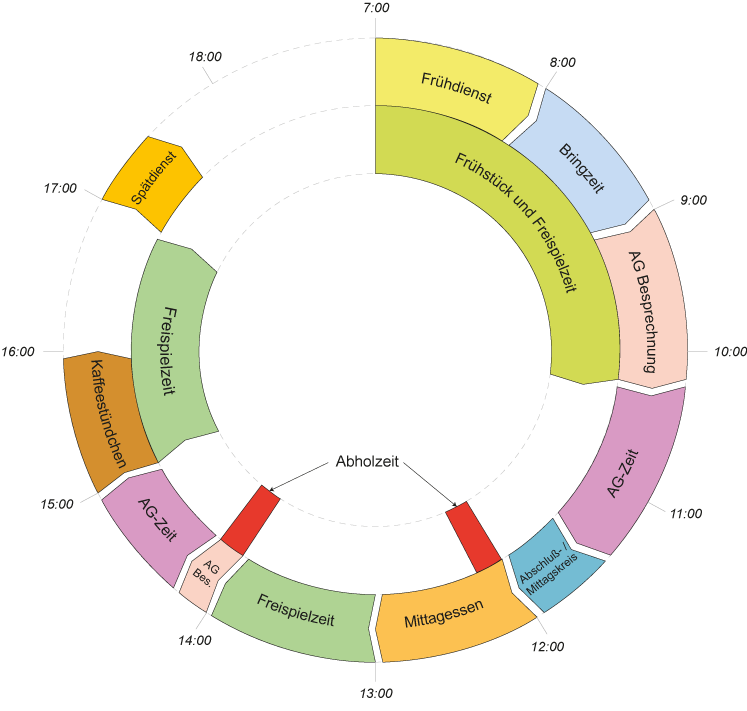
\includegraphics[width=0.82\textwidth]{grafik/tagesablauf.png}
      \captionof{figure}[Tagesablauf der Kindertagesst�tte Lotte Lemke]{Ein Beispiel Tagesablauf der Kindertagesst�tte Lotte Lemke}
      \label{fig:tagesablauf}
    \end{center}
    
  
  \section{Elternarbeit}\label{sec:7_4}
    \begin{flushleft}
      Die Elternzusammenarbeit ist ein wichtiger Punkt in der KiTa Lotte Lemke. Sie beinhaltet Erstgespr�che, Elterngespr�che und Elternabende \citep[S.~29]{Eltzuar2000}.
    \end{flushleft}
    
    \begin{flushleft}
      \textbf{Elterngespr�che}
      \\ 
      Der Informationsaustausch �ber den Entwicklungsstand des Kindes erfolgt unteranderem durch Elterngespr�che. Diese k�nnen jederzeit, nach Terminabsprache, gef�hrt werden \citep[vgl.][S.~28f]{Eltzuar2000}. Die P�dagogen bereiten sich hierf�r mit der Entwicklungsmappe des jeweiligen Kindes vor. In der Mappe befinden sich Kinderbeobachtungsb�gen (KBB) (vgl. Anhang \ref{chap:anhang_7}), Soziogramme (vgl. Anhang \ref{chap:anhang_8}), Kinderfrageb�gen (vgl. Anhang \ref{chap:anhang_9}), Entwicklungsb�gen. Au�erdem stehen die P�dagogen im st�ndigen dialogischen Austausch mit ihren Kollegen. Vor und nach Elterngespr�chen wird sich mit der Kitaleitung ausgetauscht, diese steht den jeweiligen P�dagogen jederzeit mit Rat und Tat zur Seite. Elterngespr�che sind nicht nur ein Informationsaustausch, sie dienen auch zur Beratung und wenn n�tig auch zur Vermittlung an weitere Institutionen \citep[vgl.][S.~28f]{Eltzuar2000}.
    \end{flushleft}
    
    \begin{flushleft}
      \textbf{Elternabende}
      \\
      In der KiTa Lotte Lemke werden Gesamtelternabende und Themenelternabende nach Bedarf und Interesse angeboten. Wohingegen gruppeninterne Elternabende zweimal im Jahr stattfinden. W�hrend dieser Elternabende werden (KiTa) politische, p�dagogische und inhaltliche Themen besprochen \citep[vgl.][S.~28f]{Eltzuar2000}.
    \end{flushleft}
 

  
  \section{Die Inhalte und der Umfang der Vor- und Nachbereitung}
    \begin{flushleft}
      Den P�dagogen stehen je nach Stundenanzahl drei bis f�nf Stunden Vor- und Nachbereitung zur Verf�gung. Diese nutzen sie um KBBs, Soziogramme und Entwicklungsb�gen (vgl. Anhang \ref{chap:anhang_8}) zu erstellen. Zudem schreiben sie \enquote{Lernngeschichten} f�r die Kinder, diese kommen dann in die Schreibeordner der Kinder.
    \end{flushleft}

    \begin{flushleft}
      \textbf{Schreibeordner}
      \\ 
      Jedes Kind hat im Kinderb�ro einen Aktenorder stehen, in welchem �ber das Jahr nach Wunsch des Kindes verschiedene Dinge gesammelt werden. Die Ordner stehen in einer f�r Kinder gut erreichbaren H�he, so dass sie jederzeit angeguckt werden k�nnen. In dem Schreibeordner befinden sich unteranderem Lerngeschichten, die auf der Grundlage von Beobachtungen und Fotos, von einem Erzieher pers�nlich f�r das Kind geschrieben wurden.  Nach Wunsch k�nnen die Kinder auch Gemaltes oder Gebasteltes in ihren Schreibeordner heften.
    \end{flushleft}

    

    
  \section{Die Ausfl�ge und Reisen}
    \begin{flushleft}
      \textbf{Ausfl�ge}
      \\
      Ausfl�ge sind bestandteil des t�gliche KiTa-Alltags. Dies wird den Kindern durch die Outdoorgruppe erm�glicht. T�glich gehen zwei bis vier Kinder aus den f�nf Vormittags- und Ganztagsgruppen mit. Bei der Ausflugsplanung entscheiden die Kinder mit wem und an welchen Tagen sie mitgehen. Hierbei wird versucht, den W�nsche der Kinder gerecht zu werden \citep[vgl.][S.~19]{KonzReUb2000}. Die Ausfl�ge gehen von um 9:00 Uhr --- 12:00 Uhr und f�hren die Kinder in die nahe und ferne Umgebung von Halstenbek. F�hrt es die zwei Erzieher und die 15 Kinder bis nach Hamburg.
    \end{flushleft}

    \begin{flushleft}
      \textbf{Reisen}
      \\
      Reisen finden hingegen alle zwei Jahre statt. Die Planung der Reise ist ein langer Prozess, den Kinder, P�dagogen und Eltern gemeinsam tragen. Es wird �berlegt wohin man reisen kann, so dass es sich auch alle leisten k�nnen. Wie kommt man da am Besten hin? Welches Kind m�chte bei welchem Erzieher bzw. welcher Erzieherin �bernachten. Dieser Prozess wird durch den Kinderrat dokumentiert, protokolliert und beschlossen \citep[vgl.][S.~19]{KonzReUb2000}.
    \end{flushleft}
    
    
  \section{Qualit�tssicherung}\label{sec:7_7}
    \begin{flushleft}
      Eine  Qualit�tssicherung ergibt durch den regen Austausch der P�dagogen und P�dagoginnen untereinander und mit der p�dagogischen Leitungskraft. Wie bereits in 1.5 erw�hnt, arbeiten die  Mitarbeiter in Kooperation mit Mitarbeitern der anderen AWO Schleswig Holstein gGmbH Kindertagesst�tten, in Qualit�tszirkeln um kontinuierlich das Angebote f�r Kinder und Familien zu verbessern.
    \end{flushleft}
    
    
  \section{Ern�hrung und Hygiene}\label{sec:7_8}
    \subsection{Ern�hrung in der Kita}
      \begin{flushleft}
        Ein wichtiger Bestandteil einer gesunden Entwicklung, ist eine ausgewogene und abwechslungsreiche Ern�hrung. In der Kindertagesst�tte wird dies unteranderem durch den hauseigenen Koch gew�hrleistet.T�glich wird von ihm frisch, abwechslungsreich, ausgewogen und kindgerecht gekocht, dazu geh�rt auch mal etwas S��es. Au�erdem ist er darauf bedacht, die verschieden Essgewohnheiten und Di�ten zu ber�cksichtigen \citep[vgl.][S.~27]{KonzEr2000}. Der Aufgabenbereich des Kochs umfasst mehr als nur das Zubereitung der Speisen, er k�mmert sich auch um die organisatorische Planung, die Zusammenstellung der Speisen und den Einkauf \citep[vgl.][]{ErHy2006}.
      \end{flushleft}
      
    \subsection{Die verschiedenen Mahlzeiten}
      \begin{flushleft}
        \textbf{Das Fr�hst�ck}
        \\
        Die Kinder in der Kita Lotte Lemke haben die M�glichkeit ihr Fr�hst�ck zwischen 7:00 und 10:15 Uhr im Kindercafe einzunehmen. Meistens gehen sie mit ihrer Brottasche ins Kindercafe und  machen es sich mit einem oder mehreren Freunden gem�tlich.  Hier wird sich dann unterhalten, gegessen und auch mal nach Wunsch Essen getauscht \citep[vgl.][]{ErHy2006}. Kinder mit Allergien, Diabetiker oder mit anderen Einschr�nkungen wissen, dass sie davon ausgeschlossen sind, dies wurde mit den  Kindern  Zuhause und in der Zuhausegruppe thematisiert. Au�erdem wurden alle P�dagogInnen im Haus dar�ber informiert. Mitunter haben die Kinder aus der Zuhausegruppe  eine Auge darauf, wer was essen darf. Die Kinder d�rfen sich bei ihrem Fr�hst�ck soviel Zeitlassen wie sie wollen. Wenn sie fertig sind, k�mmert sich jedes Kind eigenst�ndig darum, dass sein Geschirr und Besteck auf den Teewagen kommen \citep[vgl.][]{ErHy2006}. Der eventuell produzierte M�ll, wird entweder zur�ck in die Brotdose bzw. Brottasche oder in die vor dem Kindercaf� stehenden M�lleimer getan. Da in der Kita- wie vieler Orts --- recycelt wird, stehen links von T�r des Kindercaf�s, w�hrend der Fr�hst�ckszeit vier M�lleimer (Plastikm�ll, Papierm�ll, Biom�ll, Restm�ll). Die Aufsicht im Kindercaf� ist durch die Gruppendienste geregelt, Montags sind z.B. die P�dagogen der Windgruppe f�r die Aufsicht des Kindercaf�s zust�ndig (Die t�glich rotierende Aufsichtspflicht der P�dagogen betrifft nicht nur das Kindercaf�, sondern auch die Turnhalle und das Au�engel�nde). Im Kindercaf� steht den Kindern t�glich zu jeder Zeit ein frischer Obst- bzw. Gem�seteller, unges��ter Tee, Milch, Mineralwasser zur freien Verf�gung \citep[vgl.][]{ErHy2006}.
      \end{flushleft}

      \begin{flushleft}
        \textbf{Das Mittagessen}
        \\
        Das Mittagessen wird t�glich frisch zubereitet und um 12:00 Uhr angeboten. Die meisten Gruppen, essen in ihrem Gruppenraum, die Regentropfengruppe und die Schneeflocken essen gemeinsam im Kindercaf�. Die Kinder k�nnen selber entscheiden ob sie mitessen wollen oder nicht, wenn sie wissen dass es ihnen nicht schmeckt m�ssen sie nicht probieren. Neue Speisen werden meistens probiert,wenn es aber nicht schmeckt k�nnen die Kinder ihren Teller abr�umen und ihre Brotdose holen. Die Kinder nehmen Einfluss auf die Mahlzeiten die ihnen serviert werden- nach jedem Essen wird eine Umfrage gemacht, wie das Essen jedem einzelnen geschmeckt hat. Hierbei k�nnen die Kinder zwischen gut, mittel und schlecht entscheiden. Dies wird dann auf einer Liste mit drei unterschiedlichen Smilies (vgl. Anhang \ref{chap:anhang_10}), f�r jeden Wochentag festgehalten. Nach dem Essen k�nnen die Kinder ihre Z�hne putzen.
      \end{flushleft}

      \begin{flushleft}
        \textbf{Das Kaffeest�ndchen}
        \\
        Das Kaffeest�ndchen f�ngt um 15 Uhr gleich nach der zweiten AG- Zeit an. Die Kinder und P�dagogInnen bekommen hier die M�glichkeit eine selbst mitgebrachte Kleinigkeit im Kindercaf� zu essen. Da das Kaffeest�ndchen �hnlich abl�uft wie das Fr�hst�ck, werde ich es nicht weiter erl�utern.
      \end{flushleft}
      
    \subsection{Hygiene in der Kita}
      \begin{flushleft}
        Die Kindertagesst�tte Lotte Lemke unterliegt --- wie alle Kindertagesst�tten- den Richtlinien der HACCP (Hazard Analysis and Critical Control Points; deutsch Gefahrenanalyse und kritische Lenkungspunkte) und des Infektionsschutzgesetzes �34 IJSG \citep[vgl.][]{ErHy2006}.
      \end{flushleft}
      
      

      \begin{flushleft}
        \textbf{Personelle Schulung} 
        \\
        Die Belehrungen des Infektionsschutzgesetzes und Hygienevorschriften erfolgt von dem Tr�ger (AWO) und wird j�hrlich aufgefrischt. Der Koch bekommt zus�tzlich viertelj�hrlich beim Wirtschaftertreffen, neue Anregungen wie die Hygieneverordnung in Kindertagesst�tten umgesetzt werden kann \citep[vgl.][]{ErHy2006}.
      \end{flushleft}


      \begin{flushleft}
        \textbf{Die Umsetzung in der K�che und im Wirtschaftsraum}
        \\
        Eine der wichtigsten Regeln f�r die K�che ist, \enquote{Eltern und Kinder d�rfen die K�che nicht betreten!} \citep[vgl.][]{ErHy2006}
        Um den Richtlinien der HACCP gerecht zu werden muss die Kerntemperatur der Speisen mindestens 65�C betragen. Au�erdem wird von jeder zubereiteten Speise eine Probe entnommen, diese wird dann mit Datum gekennzeichnet und f�r 14 Tage eingefroren. Dies passiert auch mit den Speisen, die Eltern f�r Feste zubereiten und mitbringen. Da die Gefahr beiLebensmittel bei denen die K�hlkette unterbrochen wurde und von rohen Eiern, Fisch oder Fleisch zu hoch ist --- sind sie verboten \citep[vgl.][]{ErHy2006}.
      \end{flushleft}


      \begin{flushleft}
        \textbf{Die Umsetzung in den Gruppen und beim Essen}
        \\
        Die Tische, Arbeitsfl�chen und Wickeltische werden jeden Morgen von einem P�dagogen desinfiziert. Au�erdem werden einmal die Woche die Handt�cher gewechselt und gereinigt, die Reinigung gilt auch f�r die Zahnputzbecher und -b�rsten. Die Zahnb�rsten werden nach Bedarf gewechselt \citep[vgl.][]{ErHy2006}.
      \end{flushleft}

                 
% \newpage

% Kapitel 7: Umfeld der Praxiseinrichtung				
% \chapter{Das Umfeld der Kindertagesst�tte Lotte Lemke}
  \section{Daten und Fakten der Gemeinde Halstenbek und des Kreis Pinneberg}
    \begin{flushleft}
      Die Kindertagesst�tte Lotte Lemke liegt in der Amtsfreien Gemeine Halstenbek. In der Gemeinde leben 16.744 Menschen und sie besteht aus den zwei Ortsteilen Halstenbek und Krupunder. Ihre Gesamtfl�che umfasst ca.1.260 ha und liegt im gr��ten Baumschulgebiet weltweit. Durch die g�nstige Lage der Gemeinde- sie grenzt unmittelbar an die Hansestadt Hamburg - ist sie sowohl ein beliebter Wohnort, als auch Gewerbestandort \citep[vgl.][]{Halstenbek2012}.
      Des Weiteren befinden sich sechs Kindertagesst�tten \citep[vgl.][]{HalstenbekKita} und vier Schulen in Halstenbek \citep[vgl.][]{HalstenbekSchule}. Eine der vier Schulen ist die 1994 er�ffnete Japanische Schule. Diese hat einen Zuzug  japanischst�mmigender Familien beg�nstigt \citep[vgl.][]{JapSchule}.
      \\
      Halstenbek liegt im Kreis Pinneberg dieser umfassen acht St�dte, drei amtsfreie Gemeinden und 38 amtsangeh�rige Gemeinden.
      Der Kreis ist einer der elf Kreise im Bundesland Schleswig-Holstein. Zudem ist der Kreis Pinneberg teil der Metropolregion Hamburg. Er grenzt im S�den an die Elbmetropole Hamburg und dem nieders�chsischen Landeskreis Stade. �stlich vom Kreis Pinneberg liegt der Kreis Segeberg und im Norden grenzt er an den Kreis Steinburg.
    \end{flushleft}


    \begin{flushleft}
      Obwohl das Kreisgebiet, bezogen auf die Fl�che 664 qkm der kleinste Kreis ist, ist er wiederum bezogen auf die Bev�lkerungsdichte 304.065 Einwohner der gr��te Kreis \citep[vgl.][]{KPinneberg2012}. Die Bev�lkerungsstruktur im Kreis Pinneberg weicht von der Schleswig-Holsteins in einigen Bereichen ab. So sind zwar die Zahlen der unter 18 J�hrigen und der �ber 65 J�hrigen  mit 17,6\% und 21,3\% fast identisch mit dem schleswig-holsteinischen Durchschnitt, doch bei der Arbeitslosenquote kann man schon Unterschiede erkennen: die Arbeitslosenquote vom Kreis Pinneberg liegt bei 5,6\% und in gesamte Schleswig-Holstein bei 6,9\%. So liegt das durchschnittliche Jahreseinkommen mit \EUR{20 200} nicht viel h�her als der Durchschnitt vom gesamten Schleswig-Holstein mit \EUR{18 446}, aber das erwirtschafte Bruttoinlandprodukt weicht wiederum stark ab, der Kreis Pinneberg erwirtschaftet 72 097 Millionen Euro, wohingegen das gesamte Schleswig-Holstein nur 58 092 Millionen Euro erwirtschaftet. Ein Grund daf�r k�nnten die Baumschulen sein und deren europaweiter Export und die attraktive Lage als Gewerbestandort \citep[vgl.][S.~64f]{StatSH2012}.
    \end{flushleft}



  \section{Freizeitm�glichkeiten in Halstenbek}
    \subsection{Spielangebote in Halstenbek}
      \begin{flushleft}
        In der Gemeinde Halstenbek befinden sich insgesamt sechs Spielpl�tze, wovon einer sich in fu�l�ufiger Entfernung zur Kindertagest�tte Lotte Lemke befindet. Das Gel�nde ist eingez�unt und recht klein. Trotzallem findet sich hier fast alles was ein Kinderherz begehrt: Schaukeln, Rutschen, Sandkasten und eine Kletterlandschaft. Leider ist es durch die geringe Gr��e kaum m�glich Ball zu spielen. Die anderen Spielpl�tze sind durch ihre Weitl�ufigkeit auch bei �lteren Kindern sehr beliebt, man kann hier unteranderem sein Geschick auf Kletterger�sten ausprobieren, Sandkuchen \enquote{backen}, H�llen bauen, schaukeln, auf freier Fl�che Fangen und Ball spielen.
      \end{flushleft}


    \subsection{Sportangebote in Halstenbek}
      \begin{flushleft}
        Sportangebote f�r klein und gro� finden unteranderem durch den Halstenbeker TS von 1895 statt. Hier k�nnen Kinder sowohl alleine als auch mit ihren Eltern am Turnen teilnehmen. Au�erdem haben sie die M�glichkeit, zwischen modernem Kinderballett, Karate und Leichtathletik zu w�hlen \citep[vgl.][]{htsport}. Weitere Vereine die Sportangebote f�r Kinder anbieten, sind einmal der DRLG Halstenbek-Rellingen-Schenefeld, hier werden sowohl Anf�nger als ge�bte Schwimmer aus- und weitergebildet. Die Anf�ngerschwimmausbildung findet in Schenefeld und Lurup statt. Hier lernen die Kleinen nicht nur Schwimmen, sondern auch den sichern Umgang mit dem k�hlen Nass \citep[vgl.][]{hrsDlrg2012}. Fu�ball und Tennis k�nnen Kinder ab dem f�nften Lebensjahr beim SV Halstenbek-Rellingen (SVHR) erlernen. Ein besonderes Angebot, das sehr beliebt und deswegen schon lange im Vorraus ausgebucht ist, ist das Sommer-Tennis- und Fu�ballcamp. An vier Tagen in den Sommerferien finden sich Kinder und Jugendliche von f�nf bis 16 Jahren auf der Anlage ein \citep[vgl.][]{svhr}.
      \end{flushleft}

    \subsection{Kulturelle Angebote f�r Kinder in Halstenbek}
      \begin{flushleft}
        Die B�cherhalle der Gemeinde bietet Kinder und Jugendlichen die Nutzung und den Ausleih von B�chern, CDs,CD ROMs, DVDs und H�rb�chern kostenlos an. 
        F�r Kinderg�rten und Schulen bietet die B�cherhalle au�erdem noch verschiedene Angebote an, unteranderem ein Bilderbuchkino und Besuche sowie F�hrungen au�erhalb der �ffnungszeiten \citep[vgl.][]{Buchh}.
      \end{flushleft}

    \subsection{Konfessionelle Freizeitangebote}
      \begin{flushleft}
        Die evanglisch-lutherische und katholische Kirchengemeinde Halstenbek hat ein gro�es Angebot f�r Eltern und Kinder. Mittwochs wird ein offener Spieltreff angeboten, hier k�nnen Eltern mit ihren Kindern von 16 bis 18 Uhr an verschiedenen Spielangeboten teilnehmen.
        Der Kindervormittag, der jeden zweiten Vormittag im Monat stattfindet, ist ein erweiterter Kindergottesdienst, hier wird dann auch etwas zum Thema der Andacht gebastelt und es werden Kreis- und Singspiele gespielt \citep[vgl.][]{Kirch}.
      \end{flushleft}
    
    \subsection{Anbindungen an das �ffentliche Verkehrsnetz}
      \begin{flushleft}
        Der Kreis Halstenbek ist durch die beiden S-Bahn-Stationen hervorragend, sowohl von der Hansestadt Hamburg als auch von Pinneberg, zu erreichen. Die S3 Richtung Stade ist in ca. 35 min. am Hamburger Hauptbahnhof und ca. 10 min. braucht sie bis nach Pinneberg. Dar�ber hinaus fahren die Buslinien 185,186 und 585 Richtung Hamburg, Schenefeld Pinneberg und durch die Gemeinde.
      \end{flushleft}
           
% \newpage



% \chapter{Hauptteil}
%   \begin{flushleft}
%     In diesem Kapitel wird noch einmal das Problem zusammengefasst und die in der vorliegenden Arbeit entworfene L�sung vorgestellt und bewertet. Zudem soll ein Ausblick auf m�gliche Weiterentwicklungen der hier aufgef�hrten L�sung vorgestellt werden.\citep{Cohn2010}
%   \end{flushleft}